\documentclass[12pt]{extarticle}
\usepackage{graphicx}
\usepackage{setspace}
\usepackage{xcolor}
\usepackage[a4paper, total={6in, 8in}]{geometry}
\usepackage{pgfgantt}

\begin{document}

\doublespacing

\title{\textbf{Debugging Problems}}
\author{Patrick Farmer\\ Supervisor: Dr. Jonathan Dukes}
\date{\today}
\maketitle

\begin{figure}[h!]
\centering

\includegraphics[width=\linewidth]{Images/Trinity_Main_Logo.jpg}
\label{fig:logo}
\end{figure}

\begin{center}
\large A Progress Report submitted in partial fulfillment of the requirements for the degree of MAI in Computer Engineering.
\end{center}

\newpage
\title {\Huge \textbf{\textcolor{blue}{Declaration}}}

\vspace{0.5cm}
\small I hereby declare that this Progress Report is entirely my own work and that it has not been submitted as an exercise for a degree at this or any other university.

\vspace{0.5cm}
\small I have read and I understand the plagiarism provisions in the General Regulations of the University Calendar for the current year, found at http://www.tcd.ie/calendar.
\vspace{0.5cm}

\small I have completed the Online Tutorial on avoiding plagiarism `Ready Steady Write', located at http://tcd-ie.libguides.com/plagiarism/ready-steady-write.
\vspace{0.5cm}

\small I consent to the examiner retaining a copy of the thesis beyond the examining period, should they so wish (EU GDPR May 2018).
\vspace{0.5cm}

\small I agree that this thesis will not be publicly available, but will be available to TCD staff and students in the University’s open access institutional repository on the Trinity domain only, subject to Irish Copyright Legislation and Trinity College Library conditions of use and acknowledgement.
\vspace{2cm}

\small Signed:~Patrick Farmer\hfill Date:~\today

\newpage
\tableofcontents

\newpage
\section{Introduction}

Due to the developments in LLM capabilities over the past few years have introduced a couple of issues with the classic approach for teaching programming have arisen.\\
The main issue is that AI assisted programming will likely exist in every job in the coming years, meaning that being able to work effectively with AI is also a very valuable skill. This project aims to address both of these issues by creating a tool that can generate defective code which the student must then debug.\\

\section{Goals and Objectives}

\subsection{Primary Goal}

The primary goal of this project is to create a tool that can generate code with bugs in it that provide meaningful lessons for the students that are debugging it.

\subsection{Secondary Goals}

Some more specific goals for this project are:
\begin{itemize}
    \item Have the tool generate varying types of programs and types of bugs so that it tries to not give any two students the same problem. This is done by using a comparison between the generated code and if any of the files exceed some threshold they are re-generated.
    \item To the greatest extent possible prevent or detect and correct hallucinations from the model whether that be related to the initial code creation or the bug injection. This is done using some manual checking with compiling and syntax checking but is also done by re-querying the LLM with its own response to improve the quality of the response.
    \item To have the ability to generate test cases for the working code to check if the student has fixed the bug. This is done by running the working code with some inputs and saving the output to provide test cases.
    \item Attempt the bug insertion using a more controllable approach using AST.
\end{itemize}

\section{Literature Review}

Debugging has always been a crucial part of programming but many universities do not actually directly teach it. This is a problem outlined by Li in \cite{li2019}. Also as previously mentioned the need for debugging skills is much more important now that AI is becoming more prevalent in the workplace as discussed by Denny in \cite{denny2024}. The skill of debugging also has a number of sub-domains that need to be taught too as outlined in \cite{li2019} the key 3 are knowledge of the language, knowledge of the specific program being debugged and knowledge of how to debug. The latter is the skill that this project aims to teach.\\
\\
When novice programmers write code they will inevitably write bugs into their code. The approach they take to solve the bug though is almost always to make small changes to syntax and run the code again straight away and do not take the time to understand the problem as is highlighted by Jadud in \cite{jadud2006}. This is another issue the tool helps to solve, by injecting bugs that create underlying problems it will force the student to try to understand the code.\\
\\
Another aspect of the debugging process that this tool aims to teach is the use of debugging tools such as python debugger. This is mentioned as one of the sub-domains of debugging by Li in \cite{li2019}, developing the skills to use these debuggers will inevitably help the student debug in the future. However, Odell \cite{odell2017} disagrees and believes that the best way to teach debugging is to force the student to think about the program without any help from tools. The choice of whether to include debugging software can be used could be argued is best left to the professor who knows what they want to teach the students with the task they are giving.\\
\\
As mentioned by Nguyen in \cite{nguyen2024} there is a lot of potential for misunderstanding between the AI and the user, this is something particularly true for novice programmers who will have more difficulty being precise with their wording as they will not understand the problem as well. This is where there is potential for teaching students to use LLMs effectively. the plan is to include an optional feature of solving the problem using an LLM that can be turned on or off by the professor depending on the difficulty of the task. A similar approach for giving students access to LLMs is discussed by Denny in \cite{denny2023}, where it was showed that students who were limited to only using LLMs and no ability to manually change code learned how to prompt the LLM correctly.\\


\section{Current state of the project}

The tool currently will first generate code by querying an LLM to generate code for some problem. The code is then checked to make sure that it works and a couple of test cases are generated using the working code. A bug is then inserted into the code using the LLM again or by using an AST method. The code is run again and it makes sure that it fails the test cases now. The code and test cases are then given to the student inside the environment and the student can try to fix the code to pass the test cases. The tool will attempt to improve the output of the LLM using self-reflection, it will then try to improve the diversity by regenerating the problem if its similarity to the other problems exceeds some threshold.\\
Through the early stages of the project it quickly became apparent that although clear progress was being made there was no metrics to measure this progress. Due to the nature of the output it is also a little difficult to measure the quality of the output. However, a couple of metrics were selected and used to measure to progress of the project and the impact of the features added. These metrics were:
\begin{itemize}
    \item The cognitive complexity of the code generated. This was measured using the cognitive complexity metric from radon.
    \item The cyclomatic complexity of the code generated. This was also measured using radon.
    \item The retry count for the generation of working code.
    \item The retry count for the generation of the bug.
    \item The similarity of the generated code to the rest of the programs generated.
\end{itemize}
There is no necessary ideal for the complexity. That would depend on the target for the task but it is a clear indicator of whether the code is overly simplistic or massively complex. The retry count and similarity score are all better the lower that they are. Below is a graph of the difference in the metrics as features are added to the tool and the impact of each can be seen.\\
\\
\begin{figure}[h!]
\centering
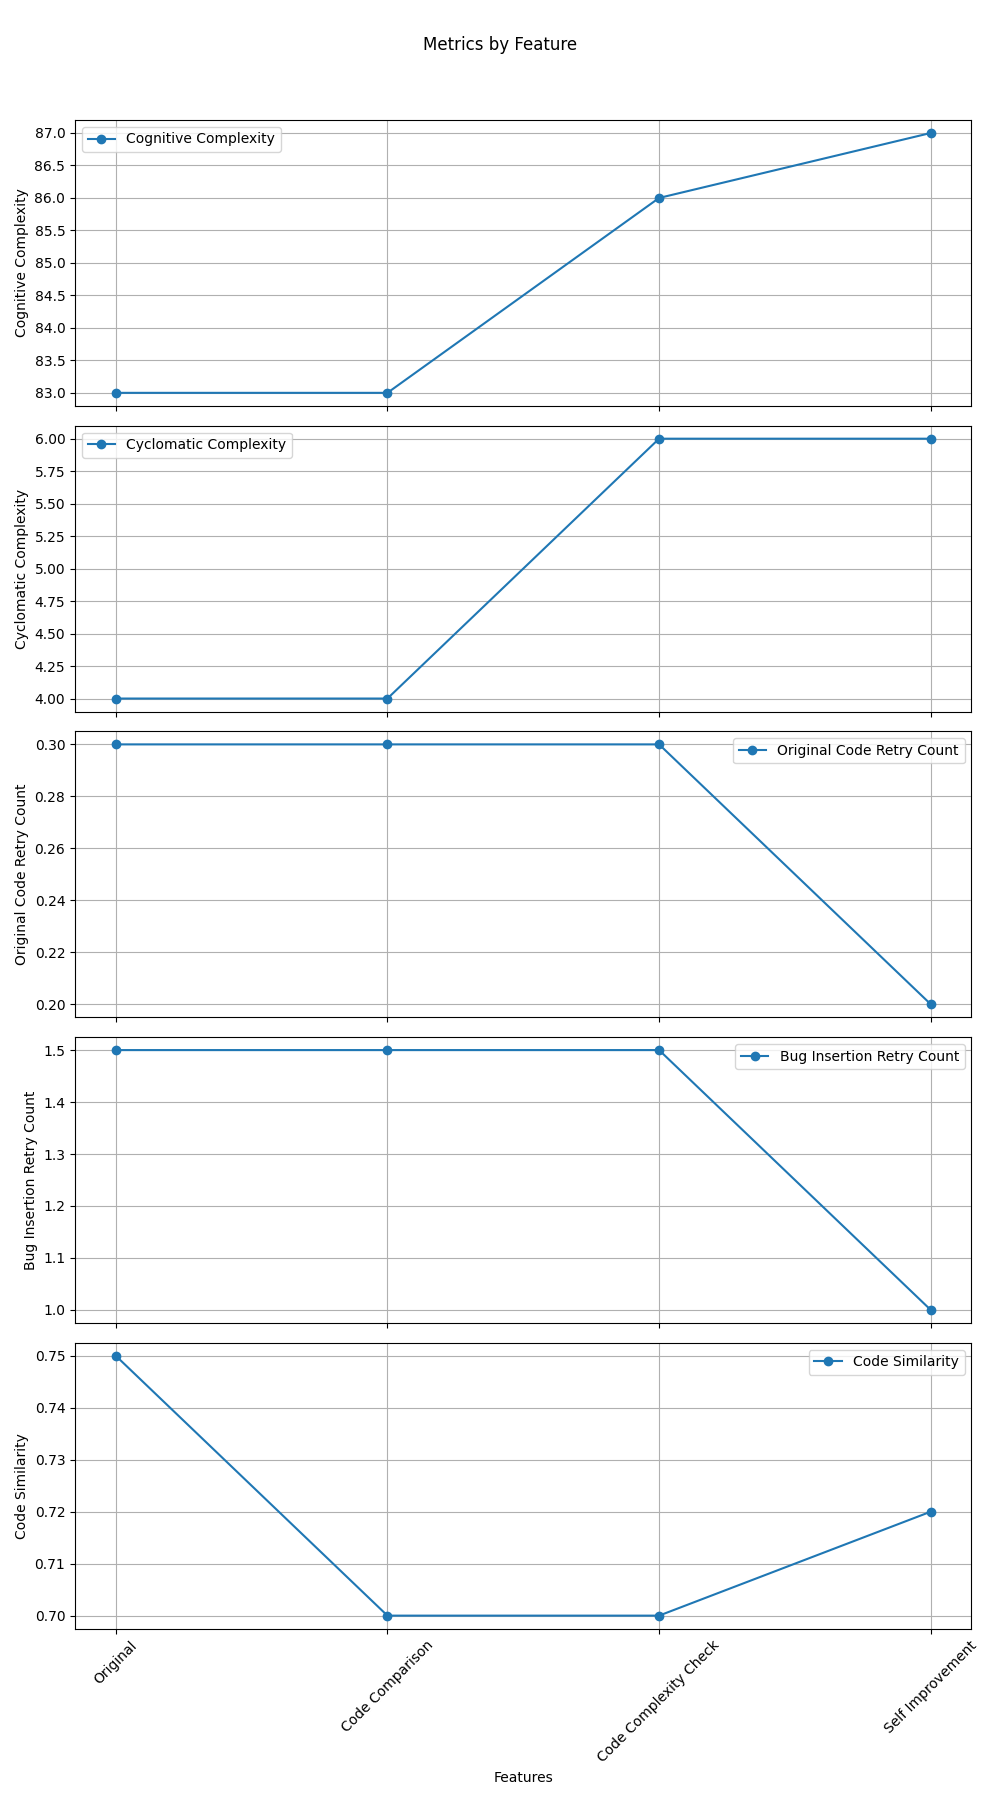
\includegraphics[width=\textwidth, height=0.8\textheight, keepaspectratio]{Images/progress_plot.png}
\label{fig:progress_plot}
\end{figure}
\\
From the above graph it can be seen that the project was seperated into 4 seperate stages. The initial project, project after code comparison was implemented, project after a code complexity check was added and the project after self improvement was implemented into the code generation class. The code comparison and complexity features improve their respective metrics a small amount. It is worth noting though that increasing code complexity is not always desirable so there is a switch to disable this feature if it is not wanted. The self improvment provides improves for the cognitive complexity and retry count metrics but reduces the diversity of the code generated.\\
\\
The issue was soon found that running the growing suit of tests for the benchmark was getting very manually intensive. For this reason there is also a pipeline setup for the benchmarking of the project that is run on a schedule via a cron job through github workflows. This allows for the project to be benchmarked regularly and the results to be stored as artifacts. The code is then run on my local machine to avoid the inevitably excessive API costs that would be incurred running the full benchmarking suite through the openAI API. There is however support for the openAI API which can be used with the flick of a switch in the command line arguments of the batch file.\\
\\
Currently the program is able to generate working code using an LLM, create one default test case, inject a bug into the code also using an LLM and ensure that the test case fails. It is the plan in the future to enable some more complex bug injection using Abstract Syntax Trees but that is not yet implemented, that is one of the significant goals for the second half of the year. Each query to the model will self reflect on itself to improve accuracy. There is also some more targeted manual checks such as making sure that the test case fails when the bug is inserted.

\section{Ethics}

The possibility of carrying out a test with real students using the tool was considering but it was instead chosen to evaluate the tool performance using desktop metrics such as those already discussed. Possible future work that might examine the impact of the tool in an academic setting may need Ethical approval but this project will not need it.

\section{Project Management}
\subsection{Risk Analysis}
There is few risks in the project as it is already in a working state just is not yet in the most mature possible state. One potential risk is the inability to add the more complex bug injection using ASTs. This is a risk because as the graph above shows the LLM has some difficulties performing the bug insertion and it would greatly increase the customisability of the bugs and the runtime of the program as it would not have to retry the bug insertion as many times. 

\subsection{Gantt Chart}
Below is a gantt chart for the project where the workload is seperated into weeks. There final stage is optional and would create a better GUI for demonstration but the essential features are the backend features outlined in the first two phases. There is also a few weeks left at the end to leave space for any unexpected issues that may arise.

\begin{figure}[h!]
\centering
\begin{ganttchart}[
    y unit title=0.5cm,
    y unit chart=0.7cm,
    vgrid,
    hgrid,
    title height=1,
    title/.style={fill=none},
    title label font=\bfseries\footnotesize,
    title label anchor/.style={below=-1.6ex},
    bar/.style={fill=blue!50},
    bar height=0.6,
    group right shift=0,
    group top shift=0.7,
    group height=.3,
    group peaks height=.2,
    x unit=0.8cm
]{1}{12}
    \gantttitle{2025}{12} \\
    \gantttitlelist{1,...,12}{1} \\
    \ganttgroup{Necessary Improvements}{1}{2} \\
    \ganttbar{Self Reflection}{1}{1} \\
    \ganttbar{Code Comparison}{1}{1} \\
    \ganttbar{More test case coverage}{2}{2} \\
    \ganttgroup{AST Implementation}{3}{7} \\
    \ganttbar{Insert any error}{3}{3} \\
    \ganttbar{Reasonable syntax error}{4}{4} \\
    \ganttbar{Underlying logic error}{5}{7} \\
    \ganttgroup{Interactable GUI (optional)}{8}{9} \\
    \ganttbar{Run code in GUI}{8}{8} \\
    \ganttbar{Run debug in GUI}{8}{8} \\
    \ganttbar{LLM sidepanel}{9}{9} \\
    \ganttbar{Default problems + manual panel}{9}{9} \\
    \ganttgroup{Deliverables}{1}{11} \\
    \ganttbar{Report}{1}{11} \\
    \ganttbar{Presentation}{2}{6} \\
\end{ganttchart}
\caption{Gantt Chart for Project Timeline}
\label{fig:gantt}
\end{figure}

\newpage
\section{Conclusion}

So far a lot of progress has been made in creating a functional tool that meets the project outline of generating problematic code that students can solve to improve their skills at debugging. The focus from here on out will be to improve some of the features that already exist to create a more reliable tool that can generate problems that are more beneficial for students. There is also scope for improvement for the presentation of the tool which I hope to address with the outlined features for GUI if time permits.\\
The tool can only do so much to address the teaching of debugging. The user will still need to setup the tool in a way that will teach the students meaningful lessons. This is why I also hope to create a set of default prompts with the tool that can be used to generate beneficial problems quickly.

\section{References}
\begin{thebibliography}{9}

\bibitem{jadud2006}
Jadud, M. C. (2006). Methods and tools for exploring novice compilation behaviour. Proceedings of the Second International Workshop on Computing Education Research, 73–84. https://doi.org/10.1145/1151588.1151600

\bibitem{li2019}
Li, C., Chan, E., Denny, P., Luxton-Reilly, A., \& Tempero, E. (2019). Towards a Framework for Teaching Debugging. Proceedings of the Twenty-First Australasian Computing Education Conference, 79–86. https://doi.org/10.1145/3286960.3286970

\bibitem{odell2017}
O’Dell, D. H. (2017). The Debugging Mindset: Understanding the psychology of learning strategies leads to effective problem-solving skills. Queue, 15(1), 71–90. https://doi.org/10.1145/3055301.3068754

\bibitem{parkinson2024}
Parkinson, M. M., Hermans, S., Gijbels, D., \& Dinsmore, D. L. (2024). Exploring debugging processes and regulation strategies during collaborative coding tasks among elementary and secondary students. Computer Science Education, 0(0), 1–28. https://doi.org/10.1080/08993408.2024.2305026

\bibitem{whalley2021}
Whalley, J., Settle, A., \& Luxton-Reilly, A. (2021). Analysis of a Process for Introductory Debugging. Proceedings of the 23rd Australasian Computing Education Conference, 11–20. https://doi.org/10.1145/3441636.3442300

\bibitem{whalley2023}
Whalley, J., Settle, A., \& Luxton-Reilly, A. (2023). A Think-Aloud Study of Novice Debugging. ACM Transactions on Computing Education, 23(2), 1–38. https://doi.org/10.1145/3589004

\bibitem{denny2023}
Denny, P., Leinonen, J., Prather, J., Luxton-Reilly, A., Amarouche, T., Becker, B. A., \& Reeves, B. N. (2023). Promptly: Using Prompt Problems to Teach Learners How to Effectively Utilize AI Code Generators. https://doi.org/10.48550/ARXIV.2307.16364

\bibitem{denny2024}
Denny, P., Leinonen, J., Prather, J., Luxton-Reilly, A., Amarouche, T., Becker, B. A., \& Reeves, B. N. (2024). Prompt Problems: A New Programming Exercise for the Generative AI Era. Proceedings of the 55th ACM Technical Symposium on Computer Science Education V. 1, 296–302. https://doi.org/10.1145/3626252.3630909

\bibitem{nguyen2024}
Nguyen, S., Babe, H. M., Zi, Y., Guha, A., Anderson, C. J., \& Feldman, M. Q. (2024). How Beginning Programmers and Code LLMs (Mis)read Each Other. Proceedings of the CHI Conference on Human Factors in Computing Systems, 1–26. https://doi.org/10.1145/3613904.3642706

\end{thebibliography}

\end{document}